\chapter{The Final Solution}
\label{chp:5:FinaSolu}
In this chapter, a final design of a mass communication system, named Myriad, will be introduced. Firstly, the improvements on the requirements will be compared to the ones defined for the prototype from previous chapter. Later, the actual product features, and its architecture will be discussed.

\section{The Improved Requirements}
\label{sec:5.1:ImprRequ}

Having seen the prototype in action made us to revise the requirements, and bring the new ones. Some of those requirements are shaped according to the feedback that we got during our research at the Stanford \ac{HCI} group, as well as from the organizations who do mass email communication on weekly basis to reach their community. In the following sections those new features of the final product will be discussed.

\subsection{Assistant Support}
\label{subsec:5.1.1:AssiSupp}
As it was described in section \ref{subsec:4.1.1:Cust}, the standard that we want to achieve within a mass email communication is the most adequately personalized emails for each recipients with minimum effort on a researcher's side. The initial idea and the prototype included several features for this purpose as discussed in chapter \ref{chp:4:InitIdeaProt} for this purpose. However, if you consider the gold standard we would like to achieve in the figure \ref{fig:ChartEffortCustom}, the prototype still leaves some effort on a researcher's side to accomplish a successful mass email campaign.
\vspace{1cm}

In order to reduce the effort as much as possible during a mass email communication, the additional assistants' involvement was considered. Therefore, a primary researcher will be able to share the tasks with permitted assistants. These might be tasks such as extracting information from the incoming answers, proofreading the primary researcher's replies before sending, or even writing replies to those answers. Hence, the primary researcher will only need to interact with the flow of a mass email campaign when there is a situation where the primary researcher's attention needed. However, the system still needs to provide the necessary features that we will see in the next sections to support the work flow in a mass email campaign, hence assistants will only need to interact with this work flow to let the continuation of the email campaign by providing answers with the email templates, and extract information as \ac{KVP}s.

\subsection{Dynamic Variables and \ac{KVP}s}
\label{subsec:5.1.2:DynmVariKVPs}
We introduced dynamic variables at the initial prototype, however it was only limited to the salutation of the email. Since it makes the personalization of emails easier, and email marketing applications also support this feature in the same way, as described in section \ref{subsec:3.3.3:EmaiMarktAppl}, the final product will also include this feature. As a result, application users can create \ac{KVP}s and use those keys in the content of an email message to be replaced dynamically by its value according to the recipient. Therefore, the extracted information from emails will not just help us to gather information in an organized way, but also use it to personalize the emails
\vspace{1cm}

As a result, instead of keeping the \ac{KVP}s in the system according to the responses, the system should keep them according to the recipients itself. This is where the \ac{KVP}-idea differs from the prototype as well. So, we have now profiles of contacts for a campaign having all \ac{KVP}s of a recipient visible during the whole state of the conversation. However, the system should offer an option to hide individual \ac{KVP}s to avoid cluttering on the view, and keep the \ac{KVP} list with the ones that are actively used.

\vspace{1cm}
Importing the \ac{KVP}s should be done in several ways. One option is that the system should be able to synchronize with an online spreadsheet, e.g. Google Spreadsheet, to get the \ac{KVP}s at the beginning of a campaign. This is a convenient way for researchers since they are already familiar with spreadsheet environments. Other options should be a campaign-wide view and a contact specific view in the system. Also, it should be allowed to edit both keys and values in a campaign.

\subsection{Importing and Exporting Contacts and Their Information}
\label{subsec:5.1.3:ImpoExpoContInfo}
In the prototype, the application user had to enter the basic information of the recipients such as first name, last name, and email address into the system manually. However, we realized while they were doing this, they use a spreadsheet and copy the contact information from there. This was also the case for their regular email client that they used for email campaigns. The applications that were investigated in section \ref{sec:3.3:Resul} had an option to import data from spreadsheet to ease the process. Therefore, the system should offer an option to import contacts from a spreadsheet environment.
\vspace{1cm}

However, importing should not only be limited to the basic information of recipients. Since we already mentioned about importing \ac{KVP}s from a spreadsheet in the previous section, the system should detect and import the contact information and \ac{KVP}s related to that contact if they are available at a provided spreadsheet. 
\vspace{1cm}

The system should provide a bi-directional synchronization, not just support to import data from the spreadsheet. Therefore, the system should provide an option to export contact information and their created \ac{KVP}s from the system to the spreadsheet. This gives a reporting functionality to the application users, where they can see all the contacts, and their extracted information from a campaign on one view.

\subsection{Interoperability with Other Email Clients}
\label{subsec:5.1.4:InteEmaiClie}
Even though we provide a new system for the users to initiate their mass email communication, there might be some cases where a mass email communication initiated in the user's regular email client, and the system is not aware of that campaign since it was not created with it. The application should provide an option to import those email messages created with another email client into the system by recognizing those messages annotated by the user.
\vspace{1cm}

Enabling the system to import email conversations from other email clients reduce the dependency on the application, and while researchers continue to use their own email clients, assigned assistants can take care of those emails imported by the researchers. We saw such an import feature in \ac{CRM} applications in section \ref{subsec:3.3.1:CRMAppl} as well, where a user is able to forward an email to the \ac{CRM} application's provided unique email addresses, and the system takes care of assigning the imported emails to the corresponding recipients in the system.

\subsection{Automated Decision-Making and Notifications}
\label{subsec:5.1.5:AutoDeciMakiNoti}
Even though the involvement of assistants makes the primary researcher's life easier, the system still needs to provide an automated approach to answer the emails whose statuses are clear in the flow of a mass email communication. Therefore, a rule based decision-making mechanism should be used, at which a user sets the values of the keys from \ac{KVP}s, and it triggers the action of sending emails to respondents whose \ac{KVP}s satisfies the provided condition.
\vspace{1cm}

Since the application's only purpose is the managing mass email communication and each campaign results great amount of messages in the inbox, the system should provide notifications regarding what should be done next for each recipients. Labels should be added to the email conversations to state whose turn is the next in the communication. For instance, by proving a label saying "You need to reply" to the application user, the state of the communication waits an action from a researcher or an assistant. In the same way the unread conversations and the conversation waiting an answer from the recipients should be also annotated in the similar way. The system should also provide email notifications to the assistants' email addresseses to notify them there is an action waiting to be taken care of.

\section{Final System}
\label{sec:5.2:FinaSyst}
In this section, we will see that how the revised and improved requirements from the previous section reflected to the final product, named "Myriad".

\subsection{Log-In and Campaigns Overview}
\label{subsec:5.2.1:CampOver}

As it was the same case for the prototype in section \ref{subsec:4.2.2:ProtSyst}, Myriad also requires a Gmail account to work with. The reason behind this is not just the popularity of Gmail, but also that Stanford University uses Google Apps by default at university wide. Therefore, each member of the university has already a Google account to use with Myriad. This also provides flexibility, because there is no registration form or sign in screen at the Myriad. All the requested Google's permissions from a Myriad's user and their descriptions can be found in appendix \ref{app:GoogPerm}.
\vspace{1cm}

After users sign in to the system, the first screen that they will see is the campaigns overview screen. All the created campaigns including the ones assigned by other user's as an assistant are shown as in the figure \ref{fig:CampaignsOverviewScreen}. It has a simple and clean \ac{UI}, deferring from regular email clients to emphasize its focus on mass email communication.

\begin{figure}[htbp]
	\centering
	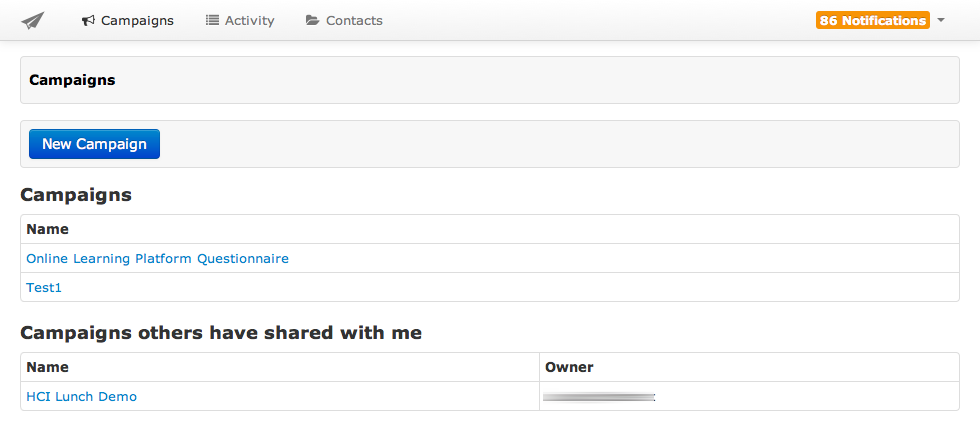
\includegraphics[width=1.00\textwidth]{imgs/CampaignsOverviewScreen.png}
	\caption[Myriad's Campaigns Overview Screen]{Myriad's Campaigns Overview Screen}
	\label{fig:CampaignsOverviewScreen}
\end{figure}

\subsection{Synchronization with Other Sytems}
\label{subsec:5.2.2:SyncOtheSyst}

Myriad is able to get the recipients' information and their \ac{KVP}s from Google Spreadsheet\footnote{https://docs.google.com/spreadsheet/}. This is a convenient way to import recipients' information into the system since many people already keep their recipients' and related information in a spreadsheet environment as we discussed in section \ref{subsec:5.1.3:ImpoExpoContInfo}. Therefore, Myriad offers a bi-directional syncing from and to the spreadsheet defined at the creation of a campaign. Besides, Myriad also has an option to enter recipients first name, last name, and email address into the system directly.
\vspace{1cm}

The corresponding columns in a Google Spreadsheet start with "first name", "last name", and "email address" as in the figure \ref{fig:GoogleSpreadsheet}. The rest of the columns will be acted as a \ac{KVP}, and imported into the system as well.

\begin{figure}[htbp]
	\centering
	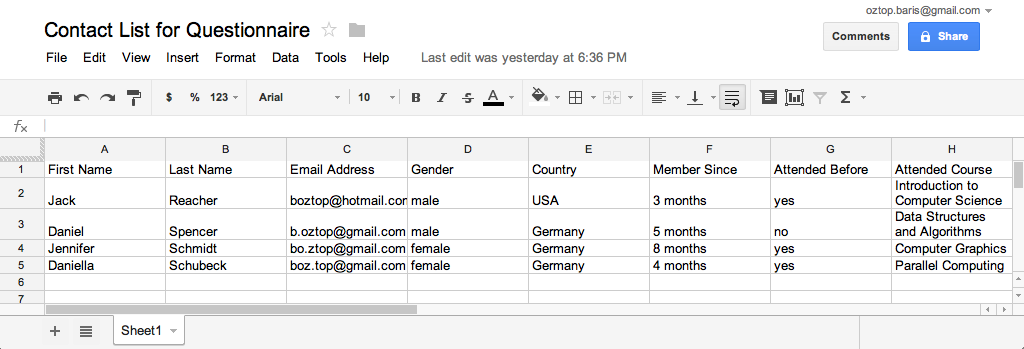
\includegraphics[width=1.00\textwidth]{imgs/GoogleSpreadsheet.png}
	\caption[A Google Spreadsheet to Import Recipients' Information into Myriad]{A Google Spreadsheet to Import Recipients' Information into Myriad}
	\label{fig:GoogleSpreadsheet}
\end{figure}

As it was mentioned in the section \ref{subsec:5.1.4:InteEmaiClie}, importing existing email conversations as a campaign message into the system is an important feature. Because, researchers may initiate conversations in their regular email client, and later on to make them more manageable, they can import them into Myriad. Myriad leverages Gmail's labeling feature which is equivalent to the \ac{IMAP} protocol's folders for this purpose \citep{GoogleInc.2013}. Myriad creates a Gmail label in the user's account, and the only thing that user needs to do is the enable label syncing feature at the campaign creation screen. Next, there will be a label same with the campaign's name, and grouped under the root label, "myriad", in the Gmail's inbox (see the figure \ref{fig:GmailLabels}). Hence, a researcher will able to import email messages, which were not considered to belong to a campaign for some reasons, into Myriad.

\clearpage

\begin{figure}[htbp]
	\centering
	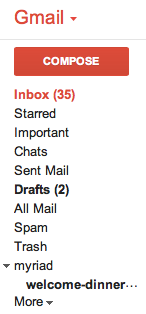
\includegraphics[scale=0.60]{imgs/GmailLabels.png}
	\caption[Gmail's Labels and Myriad's Campaigns Under the Myriad Label]{Gmail's Labels and Myriad's Campaigns Under the Myriad Label}
	\label{fig:GmailLabels}
\end{figure}

\subsection{Creating an Email Campaign}
\label{subsec:5.2.3:CreaEmaiCamp}

The campaign creation screen (see figure \ref{fig:CreateCampaign}) has input fields for a campaign name and Google Spreadsheet's \ac{URL} to synchronize with. Other two checkboxes for the spreadsheet are to manage the frequency of synchronization and disabling the cascading warning messages in case of erroneous data in the spreadsheet such as an empty email address field for a contact. The option for importing emails from Gmail's inbox is also in this screen under the label synching section.

\begin{figure}[htbp]
	\centering
	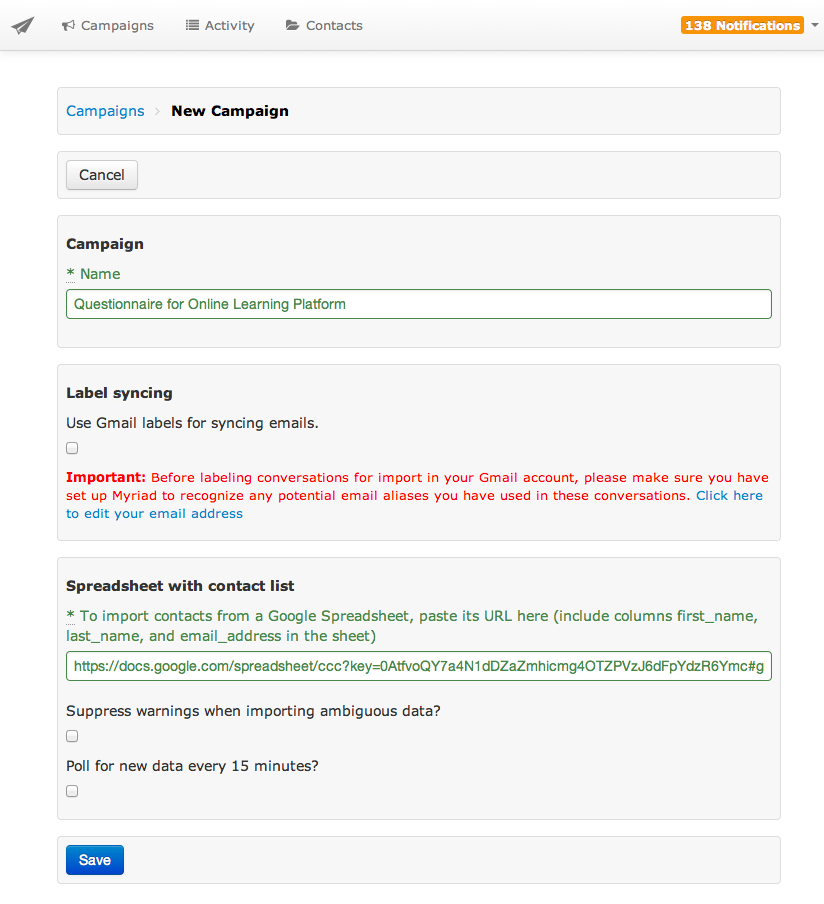
\includegraphics[width=1.00\textwidth]{imgs/CreateCampaign.png}
	\caption[Creating a Campaing in Myriad]{Creating a Campaing in Myriad}
	\label{fig:CreateCampaign}
\end{figure}

After the campaign is created, all the contacts and their \ac{KVP}s will be imported if the user provided a Google Spreadsheet \ac{URL} like in the figure \ref{fig:ContactListInCampaign}.

\begin{figure}[htbp]
	\centering
	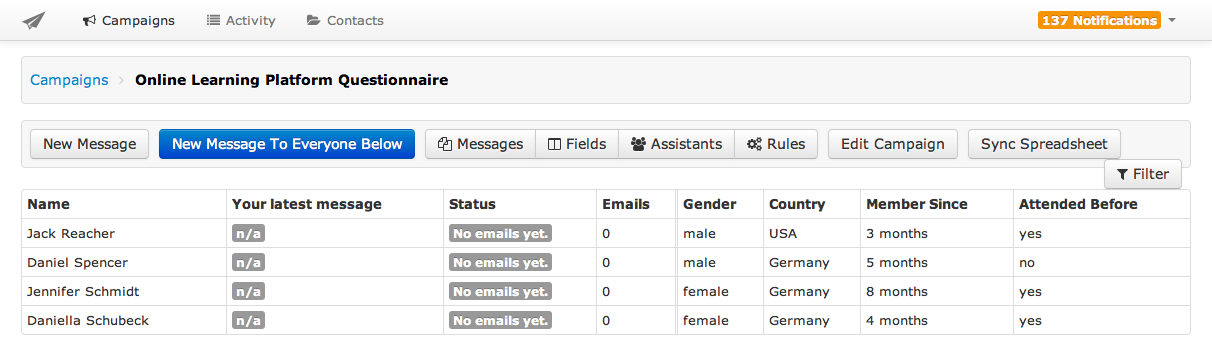
\includegraphics[width=1.00\textwidth]{imgs/ContactListInCampaign.png}
	\caption[Contacts and Their \ac{KVP}s After Synchronization in Myriad]{Contacts and Their \ac{KVP}s After Synchronization in Myriad}
	\label{fig:ContactListInCampaign}
\end{figure}

\clearpage

\subsection{Composing an Email Message}
\label{subsec:5.2.4:CompEmaiMess}

Users can send emails to all the contacts that they entered or imported into the system, or select a subset of them by using the filtering functionality as in figure \ref{fig:ContactFilters}. Provided filtering options are according to the values of \ac{KVP}s, the conversation statuses such as unread, replied, or unreplied, or the message's template names.

\begin{figure}[htbp]
	\centering
	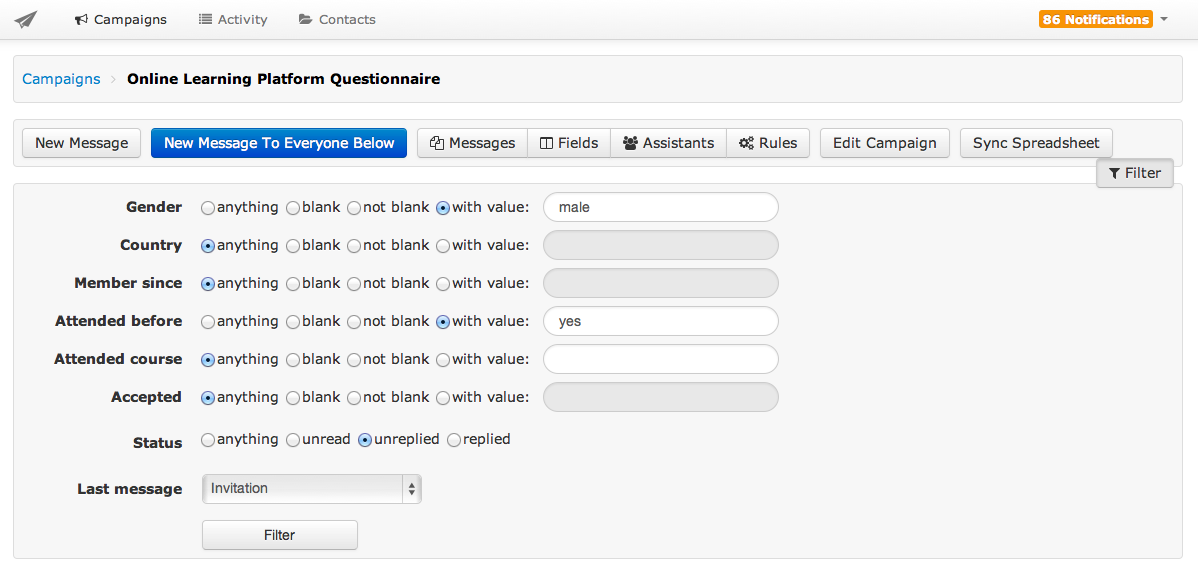
\includegraphics[width=1.00\textwidth]{imgs/ContactFilters.png}
	\caption[Filtering the Contact List in Myriad]{Filtering the Contact List in Myriad}
	\label{fig:ContactFilters}
\end{figure}

Filtered recipients are ready to compose email to them at the compose screen after pressing the corresponding button. The compose email pane (see figure \ref{fig:ComposeEmail}) contains a section that lists the previously sent emails to reuse. This is the same templating idea that was introduced at the prototype in chapter \ref{chp:4:InitIdeaProt} section \ref{subsec:4.2.2:ProtSyst}. It also shows the visualization of the state of the communication by using a tree structure, as well as the number of messages sent by using the corresponding template. A more long term campaign's visualization tree can be found in appendix \ref{app:VisuCommStat}. The system also suggest an email template while replying a responded by considering the nodes at the same tree structure.

\begin{figure}[htbp]
	\centering
	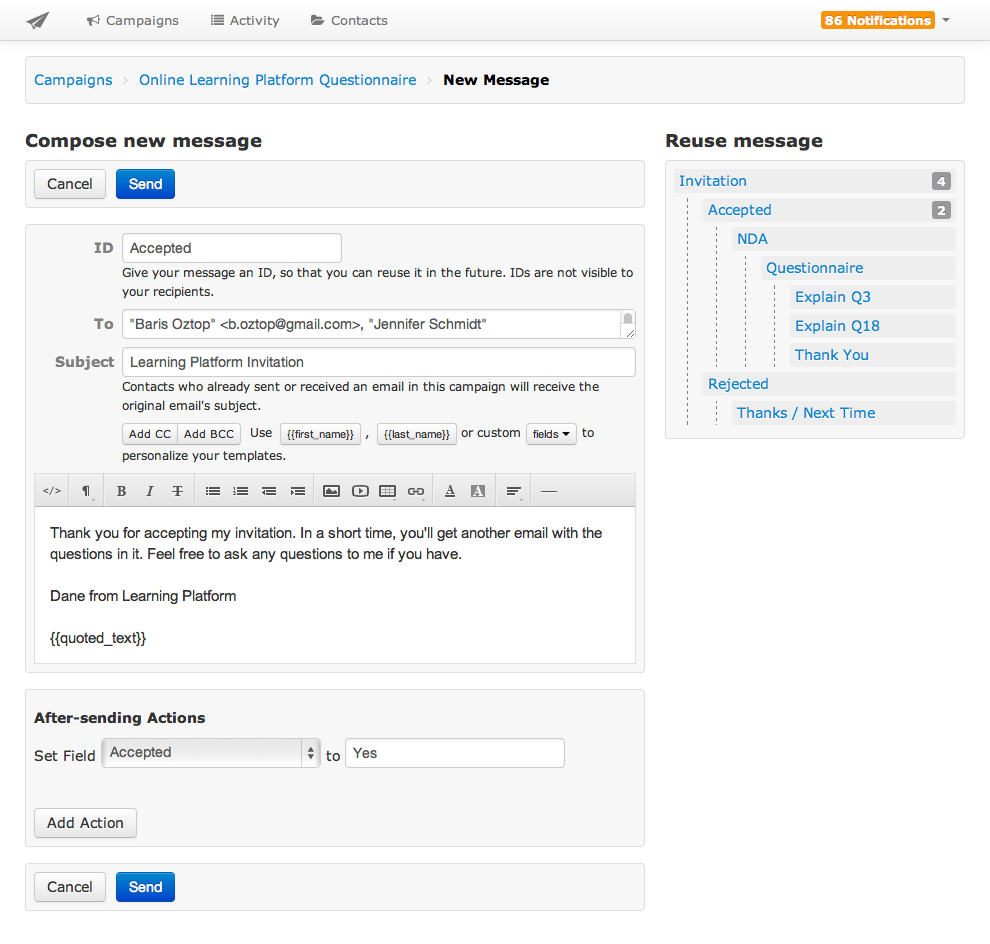
\includegraphics[width=1.00\textwidth]{imgs/ComposeEmail.png}
	\caption[Compose an Email in Myriad by Reusing Earlier Messages]{Compose an Email in Myriad by Reusing Earlier Messages}
	\label{fig:ComposeEmail}
\end{figure}

The compose pane allows users to add dynamic variables into the content of messages to personalize them according to recipients. Those variables are not just limited to the first name and last name, they can also be any keys from the assigned \ac{KVP}s in the campaign.
\vspace{1cm}

\clearpage

Each campaign has a link to the other campaigns if the recipient was involved for them too as we will see in the next section. A researcher can access to the conversations and the \ac{KVP}s from other campaigns by switching to the campaign via the provided link. Providing an option to see the earlier campaigns that a recipient involved gives broader knowledge about a recipient that may help researchers to personalize the content of the emails more easily and properly. For example, if we had extracted information regarding which sports the recipients do in an earlier campaign. We can use the same information to make a more friendly and frankly start in the new campaign by mentioning about the latest events of those sports areas in the country. Such a technique also supports the social exchange and the diffusion of responsibility theories as discussed in section \ref{sec:2.3:PersEmai}. There is also an option to hide the \ac{KVP}s in a campaign if they are not related at all or became obsolete during the flow of a campaign to avoid cluttering of them in the application's view.
\vspace{1cm}

In the figure \ref{fig:ComposeEmail}, at the pane of "after-sending actions", users are able to set the values of the keys right after an email is sent. Therefore, a user does not need to browse to another screen to change or set \ac{KVP}s whose values depends on the email that was recently sent.
\vspace{1cm}

At the beginning of this section it is mentioned that a user can filter the recipients list, and send an email to the subset of it according to the filtered condition. Myriad saves those filtered conditions under the "Rules" menu as in the figure \ref{fig:AutomatedRules} after the user sent the email. Hence, the next time if there are new emails satisfying the same conditions as before, user will notice them under the rules menu, and the earlier sent email messages can be sent to those new matching recipients automatically if user choose to enable automated option or a user can simple press the send button manually in the same screen. For example, in the figure \ref{fig:AutomatedRules}, there are 3 recipients whose "attending" key was set to "yes", and the system already recognized that we already sent an email to those whose attending, and there are new matches for the same condition recently. In this case, the user can simply press the send button, or automate the process by enabling the provided option.

\clearpage

\begin{figure}[htbp]
	\centering
	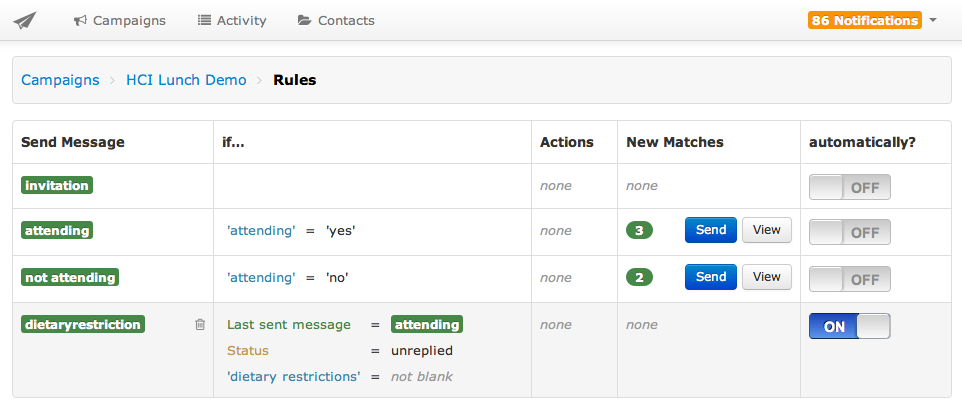
\includegraphics[width=1.00\textwidth]{imgs/AutomatedRules.png}
	\caption[Rules to Automate the Sending Process of the Emails in Myriad]{Rules to Automate the Sending Process of the Emails in Myriad}
	\label{fig:AutomatedRules}
\end{figure}

\subsection{Extracting Information from Email Messages}
\label{subsec:5.2.5:ExtrInfoEmaiMess}

Myriad's reading pane (see figure \ref{fig:MyriadReadingPane}) offers a threaded view where all the messages of a recipient and a researcher are visually grouped together. The advantage of threaded view is that it allows a researcher to get a quick overview of the whole state of a conversation, therefore a researcher can write a customized message more easily by focusing on the specific personality of the individual being respond to considering the earlier conversations with him or her at a single glance.
\vspace{1cm}

Each of the researcher's message is also annotated with the name of the message template that was used with, hence it makes the latest state of the communication easily recognizable without looking its content. In the figure \ref{fig:MyriadReadingPane}, the emails that were sent by the user had green labels writing the name of the templates that was used in it, such as "Accepted" and "Invitation" in this example.
\vspace{1cm}

While reading a recipient's answer, the extracted information can be recorded as \ac{KVP}s at the right-hand side of the reading pane (see figure \ref{fig:MyriadReadingPane}). Earlier recorded keys' values can also be updated at the same pane. Having \ac{KVP}s along with the conversation thread gives a researcher necessary information about the person that is going to be replied. Under the \ac{KVP}s pane, a researcher can also see if the recipient was involved in the other campaigns, and a link to those campaigns are provided with the amount of emails that was exchanged next to it. This is a helpful feature to remind the researcher about the existence of previous relation with the recipient, and if necessary the researcher can switch to the other campaigns to get an overview of extracted information as \ac{KVP}s.

\begin{figure}[htbp]
	\centering
	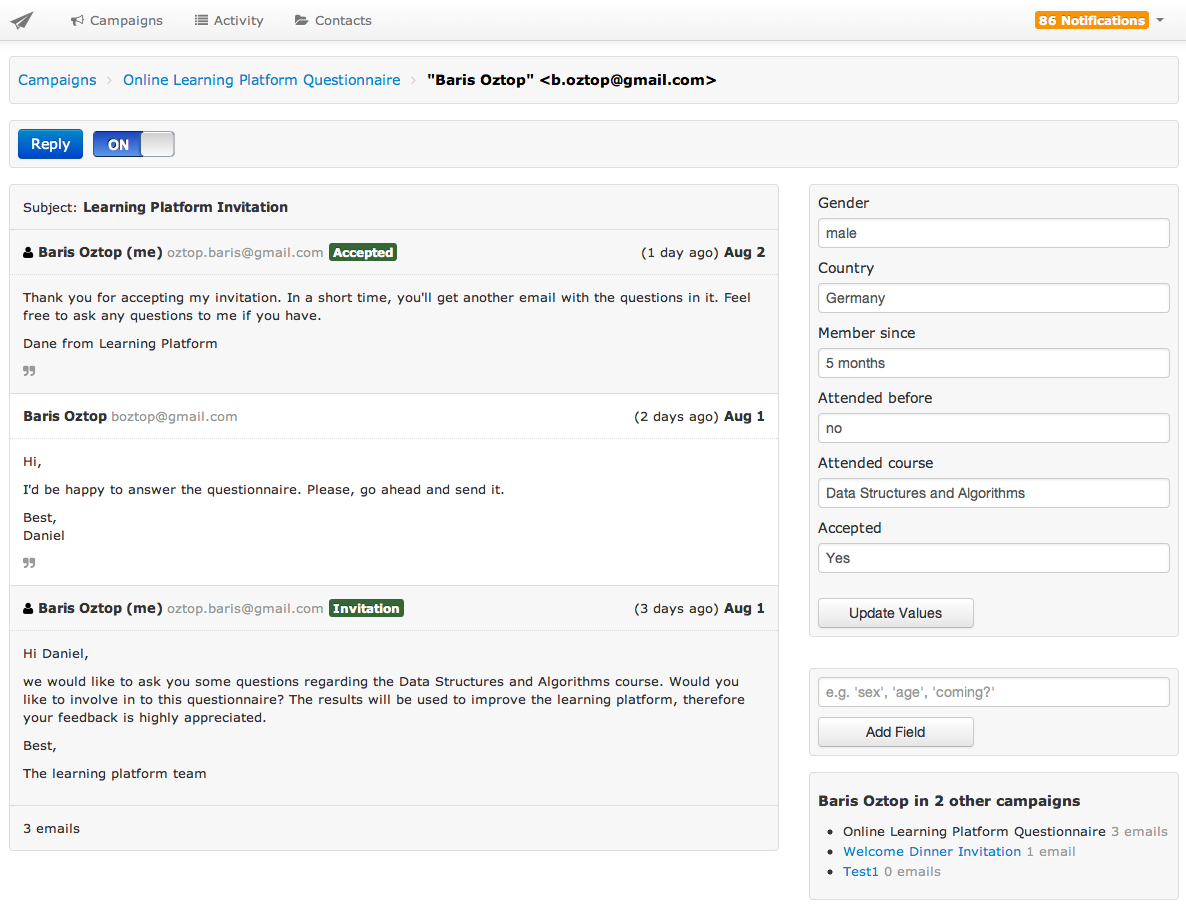
\includegraphics[width=1.00\textwidth]{imgs/MyriadReadingPane.png}
	\caption[The Reading Pane and the Extracted \ac{KVP}s in Myriad]{The Reading Pane and the Extracted \ac{KVP}s in Myriad}
	\label{fig:MyriadReadingPane}
\end{figure}

\subsection{Enabling Assistants}
\label{subsec:5.2.6:EnabAssi}

A researcher can add other researchers as assistants into a campaign by adding their Google account associated email addresses into Myriad as in the figure \ref{fig:AddAssistants}. The task of a researcher can be extracting information from emails, writing answers to the recipients, or proofreading of a researcher's emails before sending them, and many other tasks that can be generated according to the type of help a researcher needs.

\clearpage

\begin{figure}[htbp]
	\centering
	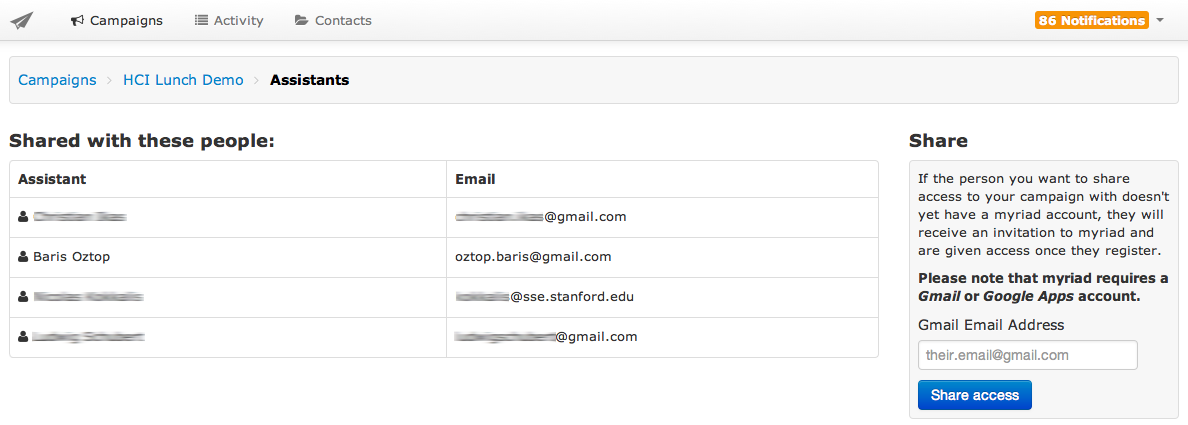
\includegraphics[width=1.00\textwidth]{imgs/AddAssistants.png}
	\caption[Rules to Automate the Sending Process of the Emails in Myriad]{Rules to Automate the Sending Process of the Emails in Myriad}
	\label{fig:AddAssistants}
\end{figure}

After an assistant is assigned to a campaign, he or she will get a notification email including the link to the campaign. Again, there will be notification emails for each email of respondents to the assistants' email address to let them know about the action required situation.
\vspace{1cm}

Myriad provides status labels for each received or sent email to give a hint about the next awaiting actions like in the figure \ref{fig:EmailStatuses}. These status labels give a hint about the next action that should be done according to the state of the conversations such as if the user needs to read or reply a message, or the conversation waits an answer from the recipient's side to continue to the communication. There are also status labels related with Myriad's internal state regarding to an email message such as if Myriad sent the messages successfully, or there was a failure with sending. The same view also provides a column to show what was the last sent message by the user. Therefore, the researchers and the assistants will easily realize what should be done next, and see the status of the communication for each recipient. 

\clearpage

\begin{figure}[htbp]
	\centering
	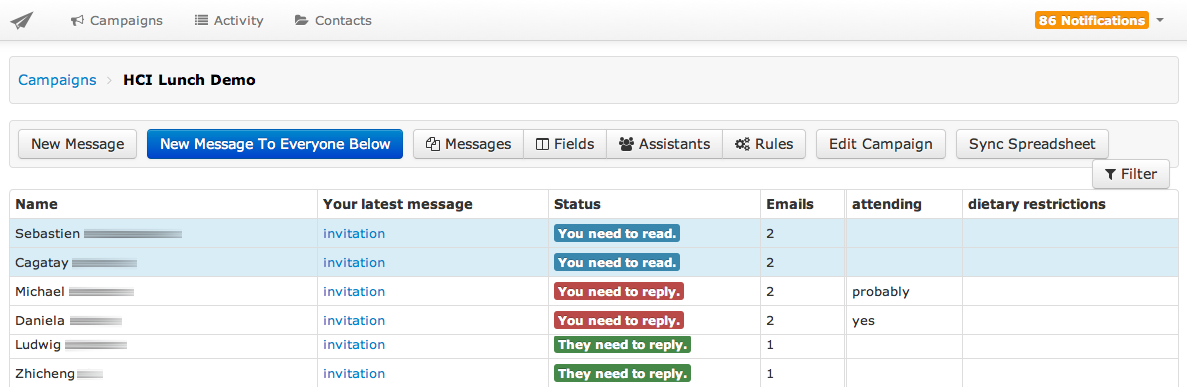
\includegraphics[width=1.00\textwidth]{imgs/EmailStatuses.png}
	\caption[Status Labels for Each Email in Myriad]{Status Labels for Each Email in Myriad}
	\label{fig:EmailStatuses}
\end{figure}

\section{Architecture}
\label{sec:5.3:FinaArch}

As it was at the prototype, Myriad was also developed using framework stack of \ac{RoR}, jQuery, Bootstrap, and OAuth\footnote{OAuth is leveraged by using OmniAuth library (https://github.com/intridea/omniauth), and its Google authentication strategy is implementation by OmniAuth Google OAuth2. Details can be found at https://github.com/zquestz/omniauth-google-oauth2} protocol was used for authentication with Gmail. Initial project structure was generated by a gem named Rails Apps Composer\footnote{https://github.com/RailsApps/rails\_apps\_composer}, which consists a collection of Rails application templates to start a project. Thanks to the other gems that we used along the way of the development to make this project completed on time in a robust way. In the next sections, we will see the implementation details of Myriad, and how it makes a mass email communication possible.

\subsection{Keeping Track of Recipients}
\label{subsec:5.3.1:ReciCont}

It was mentioned in section \ref{sec:4.2:Prot}, the prototype didn't keep information regarding to the recipients, but about the messages that they sent. Therefore, the extracted information, which are \ac{KVP}s, was related to the email messages of the recipients. The side effect of this approach was not the able get all the \ac{KVP}s of the recipients at one glance instead browsing by the earlier emails of the recipients, and each time we had to create the same key for each recipients since the system was not aware if it was already created for other email in the same campaign.
\vspace{1cm}

In Myriad, we overcame this issue by keeping all the recipients information in a separate data model named contact as in the figure \ref{fig:UML_Draw_Final}. Hence, we are able to keep track of recipients among different campaigns via the conversations of them, which is another data model in the Myriad as each campaign has many conversations of a recipient.
\vspace{1cm}

Myriad keeps the basic profile information of the recipients which are the first names, last names, and email addresses. Those information can be imported into Myriad by the spreadsheet synchronization, by adding them into "To" filed when user compose an email, or by importing from Gmail's inbox via the label synchronization. The recipients' email addresses are unique identifier for Myriad to compare already existing recipient information with the synchronized ones. 

\begin{figure}[htbp]
	\centering
	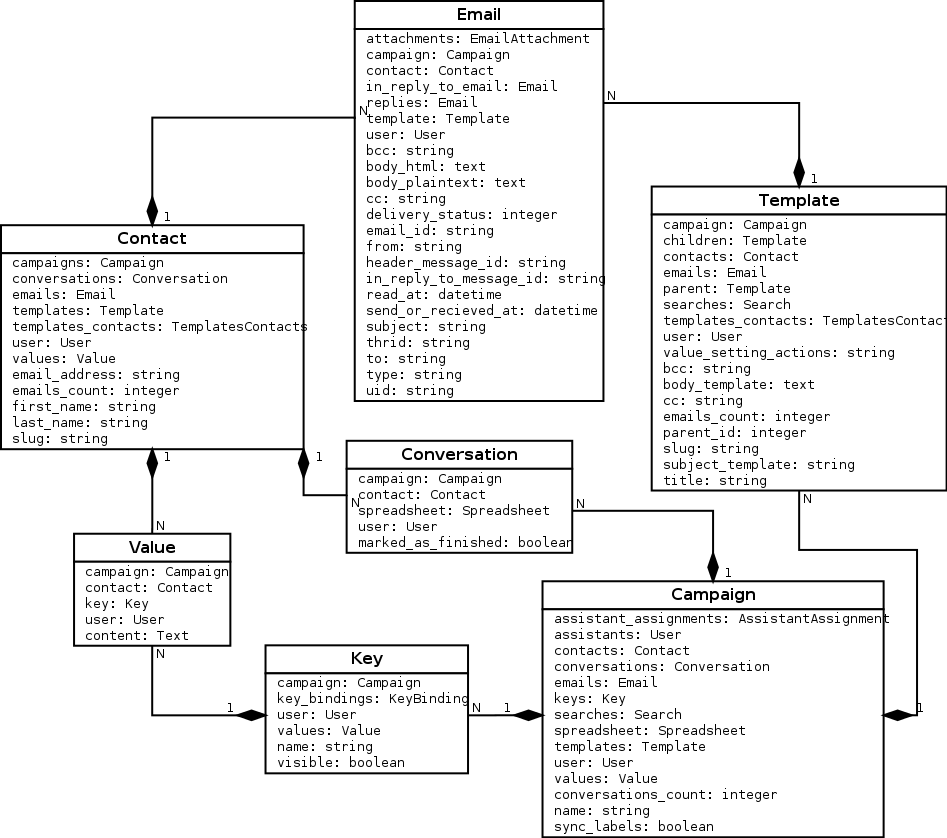
\includegraphics[width=1.00\textwidth]{imgs/UML_Draw_Final.png}
	\caption[Model Dependency of the Myriad Compared with the Prototype]{Model Dependency of the Myriad Compared with the Prototype}
	\label{fig:UML_Draw_Final}
\end{figure}

\subsection{The \ac{KVP}s and the Templates}
\label{subsec:5.3.2:KVPsTemp}

Having a separate contact data model to keep track of recipients also made us to relate each extracted information, namely \ac{KVP}s, to them, instead of their message in a campaign as in figure \ref{fig:UML_Draw_Final}. Each campaign has many keys, and their values are according to recipients. One advantages of this is when we browse to a conversation of a recipient, we are able to see all the \ac{KVP}s of that recipients under one view, which was the \ac{KVP} pane next to the email threads in the figure \ref{fig:ComposeEmail}. The other benefit comes at the synchronization with spreadsheet. When a new key is added to a recipient or a value of a key is updated via Myriad, it will be reflected to the spreadsheet as well. Therefore, the spreadsheet will always contain the latest changes done by user in Myriad. 
\vspace{1cm}

As it was in the prototype, the templates contains emails messages with dynamic variables in it, and the actual emails whose dynamic variables are filled with values are kept in the Email data model as in the figure \ref{fig:UML_Draw_Final} after they are fetched from Gmail.
\vspace{1cm}

To visualize the state of the conversation, and let the users select templates, Myriad offers the tree structure as it was in the prototype. However, the implementation of the tree structure is different from the prototype. In section \ref{subsec:4.2.3:ProtArch}, it was mentioned that the hierarchy between the nodes of the tree was a nested set model. We decided to use adjacency list model instead of nested set model to increase the readability of the templates' relation at the data model level from the developers' perspective. Since the relation of the templates is not as completed as in other relations, the performance drawbacks on this decision was negligible. 

\subsection{A Campaign Message Identification}
\label{subsec:5.3.3:MessIden}

At the prototype, due to dependency on the existing EmailValet's email fetching process, we were identifying the emails which belongs to a campaign, then inserting them into the same inbox in EmailValet. With Myriad, we removed this dependency, and only consider and show the emails which belongs to a campaign.
\vspace{1cm}

The identification of the emails depends on the three different conditions:

\begin{compactenum}
	\item The emails that are fetched from Gmail and reply to one of to the campaign message.
	\item The emails that are composed in Myriad as a part of the campaign whether they are the emails to initiate a campaign or replies to the recipients' emails.
	\item The emails that are imported into Myriad from Gmail's inbox via label synchronization (see section \ref{} for label synchronization)
\end{compactenum}

Myriad initially retrieves all the email's \ac{UID}s\footnote{UID (Unique Identifier) is 32-bit integer value to uniquely identify emails in a mailbox in \ac{IMAP}. Each email added into mailbox will have a higher value than the ones added before, however they are not necessarily contiguous \citep{rfc3501}. \ac{UID} is used as it was in the prototype by the implementation of the EmailValet's part. It is used to identify if a message is already fetched from Gmail, if it is not, it is fetched since it is a new message.} from Gmail's inbox of the last 14 days instead of all the emails of the inbox to reduce the time consumption of the fetching process. For those \ac{UID}s whose not stored in Email data model in Myriad, Myriad retrieves the actual email along with the metadata such as Gmail thread ID\footnote{Gmail thread ID is a 64-bit integer that is part of the provided Gmail's IMAP extension. It helps to associate groups of messages in the same manner as in the Gmail web interface \citep{GoogleInc.2013a}.} and Gmail labels.
\vspace{1cm}

As it was in the prototype, we set a message-ID to the emails that are composed in Myriad. Therefore, we are able to identify during the aforementioned fetching process whether an email from Gmail is the one that was composed to initiate a campaign or was a reply to the one of the recipients email in a campaign by a Myriad user. Message-ID field is again leveraged for identifying the recipients messages belonging to a campaign. Myriad retrieves the Message-ID written in the In-Reply-To, and checks if it matches one of the campaign messages in Myriad. Another field that Myriad checks is the "References" field\footnote{Reference field in another identification field along with Message-ID defined by RFC 5322. It contains one or more Message-IDs used when creating a reply to a message to identify the original message or the other messages when a reply to a message that was itself a reply \citep{rfc5322}.} to identify the messages belongs to a campaign but forwarded to another person by the recipients in order to reply the message. Since the forwarded endpoint's email client sets the Message-ID of the forwarded message into the In-Reply-To, which is not known at all by Myriad, Myriad checks the "References" field to identify a Message-ID that belongs to a campaign in this case. This scenario is illustrated in the figure \ref{fig:drawingMessageReferences}.

\begin{figure}[htbp]
	\centering
	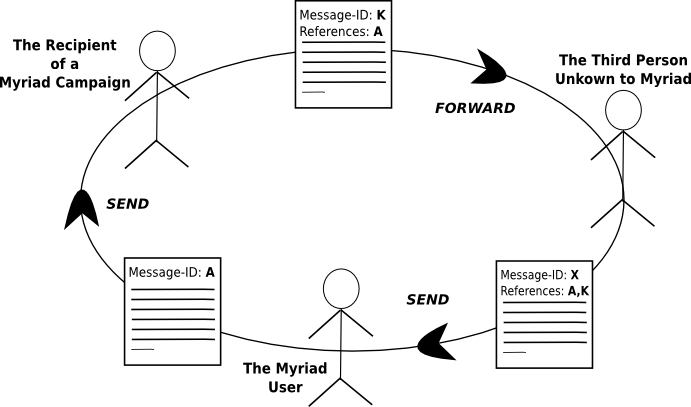
\includegraphics[width=1.00\textwidth]{imgs/drawingMessageReferences.png}
	\caption[A Scenario Using References Field in an Email]{A Scenario Using References Field in an Email}
	\label{fig:drawingMessageReferences}
\end{figure}

If an email is not identified as a campaign message by comparing the Message-IDs with the ones in Myriad's Email data model, the next step is to evaluate those emails in case of they were labelled as a Myriad campaign in the Gmail's inbox. In this case, if an email has a label in the pattern of "myriad/campaign-name", and there is already a created campaign in Myriad with the name "Campaign Name", that email will be stored in the data model. Finally, an identified email will be assigned to a contact by looking its parent email's Message-ID if it was a reply or if it fails the contact information will be recorded from the email's "From" header field. The rest of the emails will be ignored since there were no matches found in the mentioned email header fields, which are Message-ID, In-Reply-To, and References, or Gmail's Label.

\section{The Benefits of the Final Solution}
\label{sec:5.4:BeneFinaSolu}

sdfs

\begin{figure}[htbp]
	\centering
	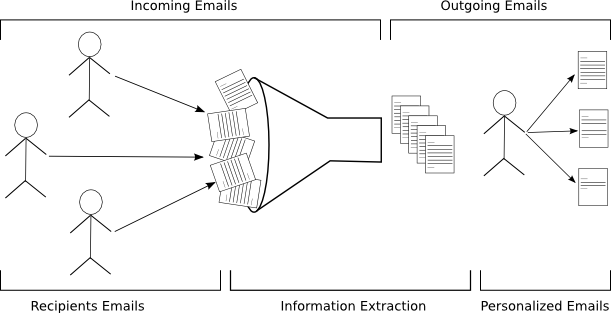
\includegraphics[width=1.00\textwidth]{imgs/drawingStatesOfEmailCommunication.png}
	\caption[A Scenario Using References Field in an Email]{A Scenario Using References Field in an Email}
	\label{fig:drawingStatesOfEmailCommunication}
\end{figure}

\section{Experiences}
\label{sec:5.5:Expr}

To date, Myriad has 67 users since its beta launch\footnote{Beta version of Myriad was launced at http://gv.stanford.edu/ and still accessebile from this address.} at January 30, 2013. Among those 67 users, 30 of them is actively using it since last month. In this section, there will be given statistics about the created campaigns and users' profile, and continued with some user's testimonials.

\subsection{Statistics}
\label{subsec:5.4.1:Stat}

The beta launch of Myriad has been advertised at the Stanford \ac{HCI} group and some Stanford's organizations who do mass email communication regularly with their communities. Some of those campaigns', and which features of Myriad they used in those campaigns are following:

\begin{compactitem}
	\item \textbf{Invitation to an Event:}User created an initial invitation template, and another template for those who rejected the invitation to motivate for the upcoming events.  Contact list is imported via spreadsheet. User also created \ac{KVP}s to differentiate the recipients who needs individual follow up. Salutations of the emails are personalized by first name \ac{KVP}.
	\item \textbf{Survey via an External Link:} User send initial template including a link to an external survey. A detailed list of contact information was imported from a Google spreadsheet. Later on, user continued with a reminder email in a separate campaign.
	\item \textbf{Importing via Gmail Labels} One of the user imported a campaign emails from his Gmail account to Myriad via label synchronization, and continued to campaign in Myriad.
	\item \textbf{Interview Results} One user reached nearly 500 recipients via Myriad to let the result of an interview process. User created a rejection template for those who were rejected, and for the ones who were accepted, he created several templates depending on the invitation date including specific schedule related to that date. The user also automate the email sending process by the created rules on the filtered search results.
	\item \textbf{Getting User Details via Form} During one of the live demonstration of Myriad at Stanford \ac{HCI} group, we asked to the attendees to browse a link to fill a Google Form\footnote{https://docs.google.com/forms} to get their contact information in a Google Spreadsheet, where the aggregated data is recorded in Google Form by default. Therefore, we were easily able to import contact information into Myriad, and initiate a campaign. There were also 4 assistants extracting information during the live demonstration while recipients were sending answers.
\end{compactitem}
\vspace{1cm}

After reviewing some use cases of Myriad, the following paragraphs will give usage statistics regarding Myriad starting from its beta launch date, January 20, 2013 till the beginning of August 2013.

\paragraph{Campaigns and Their Number of Recipients} The figure \ref{fig:ChartCampaignsRecipients} shows campaigns\footnote{Campaigns' names are removed due to privacy reasons.} created by Myriad, and their number of recipients. The average of the recipients amount was 105.32, and the total number of recipients were 9585. While the maximum amount of recipients for one campaign was 752, the minimum amount was only one recipient.

\begin{figure}[htbp]
	\centering
	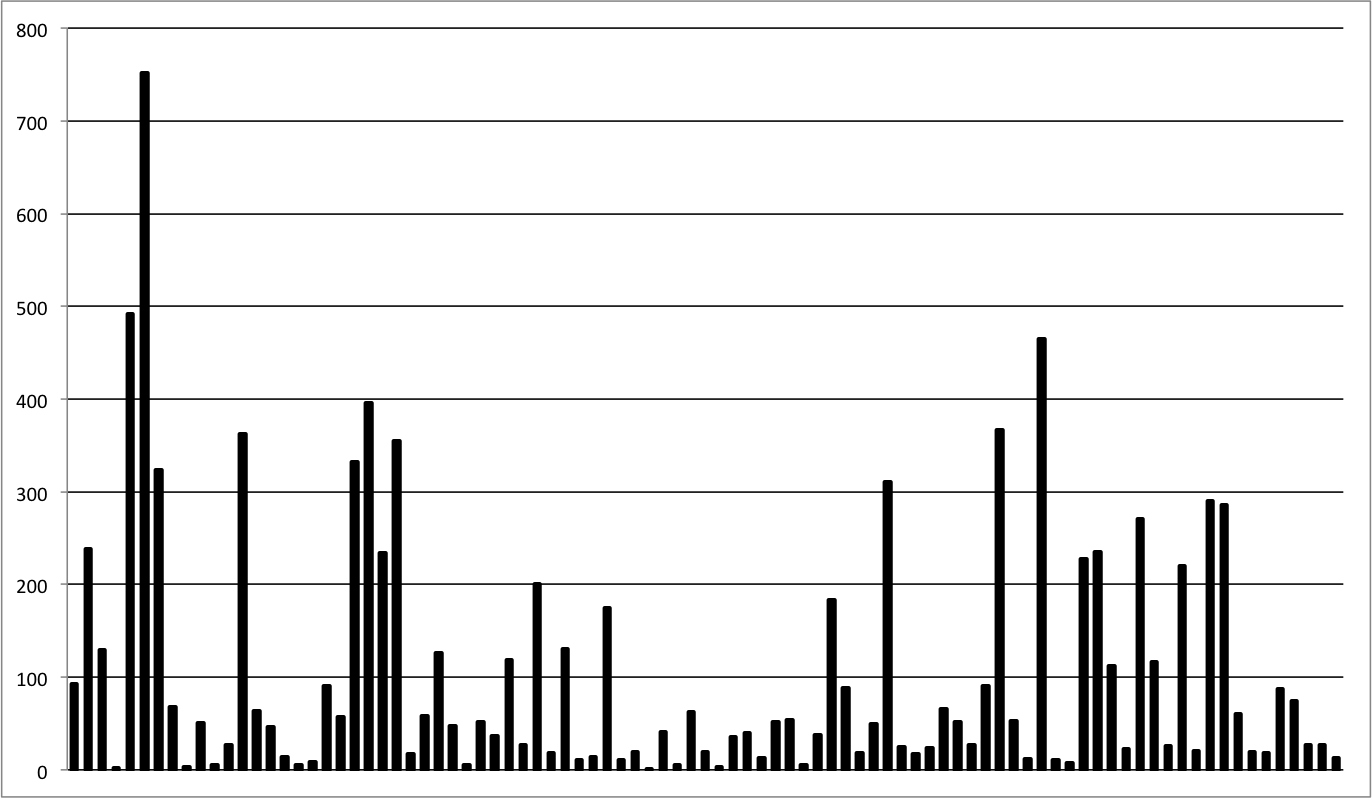
\includegraphics[width=1.00\textwidth]{imgs/ChartCampaignsRecipients.png}
	\caption[Campaigns and Their Number of Recipients in Myriad]{Campaigns and Their Number of Recipients in Myriad}
	\label{fig:ChartCampaignsRecipients}
\end{figure}

\paragraph{Myriad Users and Their Number of Campaigns} The figure \ref{fig:ChartUsersCampaigns} shows Myriad's users\footnote{Users' names are removed due to privacy reasons.}, and the number of campaigns that they created with Myriad. There are total 96 campaigns after the ones created for test purposes were ignored. The average was 3.92 campaigns per user. While the maximum amount of campaigns created by one user was 13, the minimum amount was one campaign.

\begin{figure}[htbp]
	\centering
	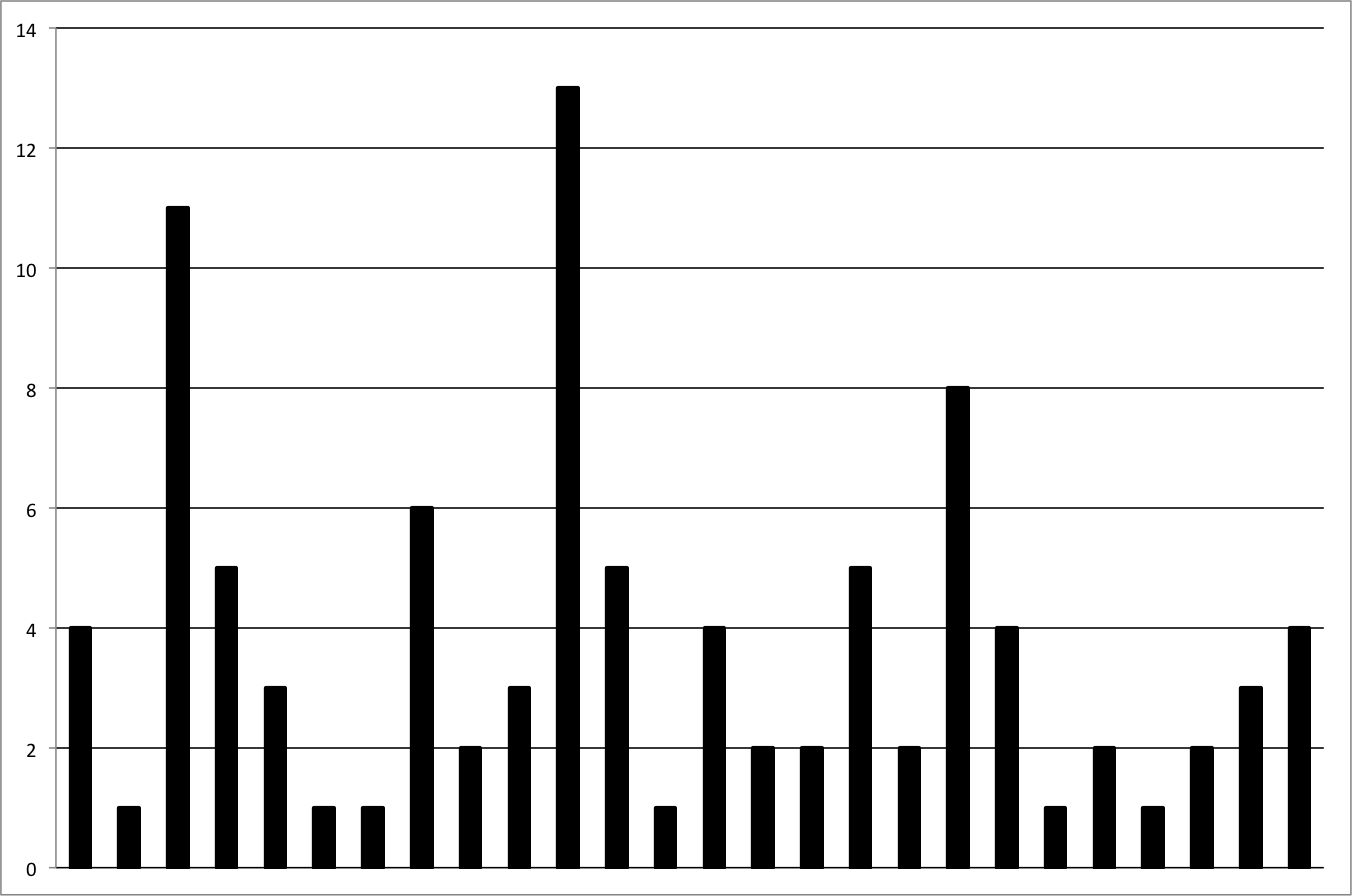
\includegraphics[width=0.85\textwidth]{imgs/ChartUsersCampaigns.png}
	\caption[Myriad Users and Their Number of Campaigns]{Myriad Users and Their Number of Campaigns}
	\label{fig:ChartUsersCampaigns}
\end{figure}

\paragraph{The Number of Campaigns per Month} The figure \ref{fig:ChartCampaignsMonths} shows the ratio of created campaigns per month. 35 campaigns out of 96 were created in April 2013 as the highest amount compared to other months. It might be because it is the middle of spring quarter at Stanford where lecturers and organizations reaches their recipients more often. There were average 15.5 campaigns create per month if the launch month January is ignored.

\begin{figure}[htbp]
	\centering
	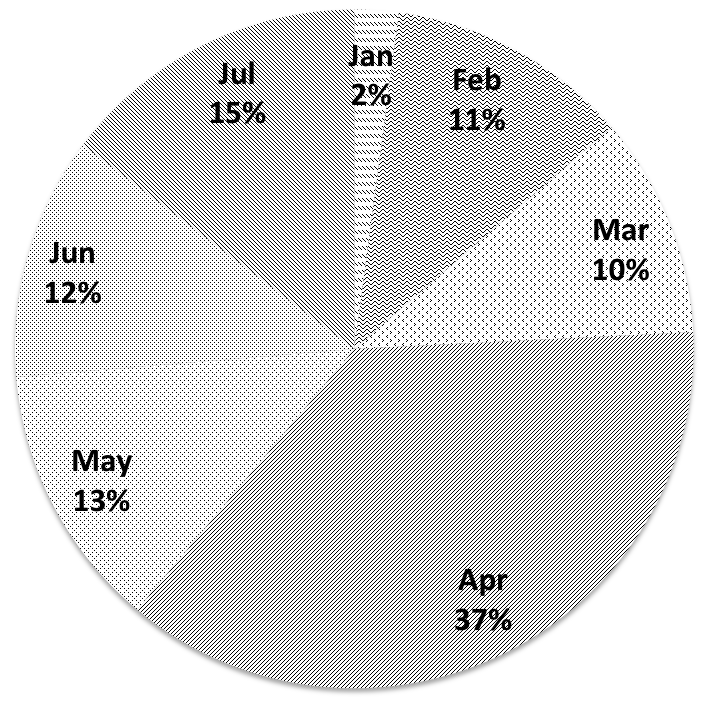
\includegraphics[width=0.48\textwidth]{imgs/ChartCampaignsMonths.png}
	\caption[The Number of Campaigns per Month]{The Number of Campaigns per Month}
	\label{fig:ChartCampaignsMonths}
\end{figure}

\clearpage

\subsection{User Testimonials}
\label{subsec:5.4.2:UserTest}

In this section,testimonials from the very active users of Myriad will be evaluated. Users were asked to evaluate Myriad keeping the following four questions in mind:

\begin{compactenum}
	\item What are the scenarios you use Myriad for?
	\item What were you using before Myriad?
	\item How satisfied are you with Myriad?
	\item How regularly you use Myriad?
\end{compactenum}

Testimonials written in listing \ref{lst:Testimonial1} and \ref{lst:Testimonial2} belongs to lecturers from Stanford \ac{HCI} group. The last testimonial belongs to a Stanford organization who do mass email communication very often to reach their community.

\vspace{1cm}

\lstset {
 basicstyle=,
 frame=shadowbox,
 rulesepcolor=\color{black},
 showspaces=false,showtabs=false,tabsize=4,
 numberstyle=\tiny,
 captionpos=b,
 xleftmargin=0.7cm, xrightmargin=0.5cm,
 lineskip=-0.1em,
 abovecaptionskip=1\baselineskip
}

\begin{lstlisting}[language=, caption={[User Testimonial \#1 about Myriad]User Testimonial \#1 about Myriad}, label={lst:Testimonial1}]

My main use: handling a special issue. Several hundred emails (literally) meant that an email view was impossible. Myriad's structured view makes everything a whole lot easier. It still needs some polishing to be ready for prime time (like it's workflow emphasis is a little constrained, and it needs better handing of formatting and attachments), but as a first draft, it's amazing. I hope it continues so I can use it more!

- Scott R. Klemmer, Stanford HCI Group
\end{lstlisting}

\vspace{1cm}

\begin{lstlisting}[language=, caption={[User Testimonial \#2 about Myriad]User Testimonial \#2 about Myriad}, label={lst:Testimonial2}]

I use Myriad to manage a large volume of emails about the courses that I'm teaching. I tag the email with the campaign, and the system+assistant help me respond with one of a number of common responses.

- Michael S. Bernstein, Stanford HCI Group
\end{lstlisting}

\vspace{1cm}

\begin{lstlisting}[language=, caption={[User Testimonial \#3 about Myriad]User Testimonial \#3 about Myriad}, label={lst:Testimonial3}]

I use Myriad when I'm mass-mailing a group of people and want to personalize the email. Before, I was using Mailchimp or BCC everyone. It's a great tool to send personalized emails to the network! I use Myriad whenever I need to email more than 10 people and want to personalize the emails.  For less than 10, the set up for Myriad may take longer than sending out the emails individually (this was discovered through trial and error).
\end{lstlisting}

\section{Conclusion}
\label{sec:5.5:Conc}

In this section, the final solution, Myriad, for mass email communication was investigated. We, first, investigated the improved requirements comparing with the initial requirements, and the ones already applied to the prototype. Enabling assistant support, using \ac{KVP}s as dynamic variables in the email, importing recipients list from Google Spreadsheet, ability to import email from Gmail's inbox by annotating email by myriad's campaign labels, and automated decision-making via previously applied search filters were some of the main improvements done in Myriad.
\vspace{1cm}

Section was continued with showing how those features are reflected on the Myriad's \ac{UI}, and followed by its introducing the architecture of Myriad on how it was possible to enable those features to support mass email communication.
\vspace{1cm}

Finally, the user and campaign statistics were given to show how actively used Myriad in its beta stage, and the section was followed by testimonials from active users of Myriad.
\vspace{1cm}

In the next section, we will see the possible extensions on the requirements on Myriad as future work, and conclude this study.

\begin{comment}

-- type of the campaigns
-- date vs number of campaign
-- date vs number of users
-- campaign Vs number of recipients
- ignore test campaigns but mention it

--> Gmail labellari ni anlatirken, diger urunlerde import nasil email forwardingle yapiliyordu onu anlat kesin.


However, we still needs to supply a system, where it offers a work flow to make it happen. satisfy these 

distribution of the work

initial idea is reducing effort as we disscussed


Requirements'dan once urunu tanit screenshot'larla cunku cok zaman kaybedecen


write first about the revised requirements,
then describe the product with pictures,
then some technical details


-------------
chapter 6 Conclusion and Future Work
-------------
Evaluation
- Experiences
- Statistics
- Conclusion

\end{comment}
